\documentclass[11pt]{article}
\usepackage[margin=1in]{geometry}
\usepackage{amsmath,amssymb}
\usepackage{graphicx}
\graphicspath{{figs/}}
\usepackage{booktabs}
\usepackage{float}
\usepackage[hidelinks]{hyperref}
\usepackage{parskip}
\setcounter{topnumber}{3}
\setcounter{totalnumber}{4}
\renewcommand{\topfraction}{0.92}
\renewcommand{\textfraction}{0.08}
\renewcommand{\floatpagefraction}{0.8}

\title{A Physics-Informed Graph Neural Network Surrogate for the 1D
Heat-Shield Solver}
\author{Grey Goodwin \\ University of Kentucky \\ grey.goodwin@uky.edu}
\date{\today}

\begin{document}
\maketitle

\begin{abstract}
This report describes a fast surrogate for the 1D heat-shield material-response
solver. The surrogate is a graph neural network trained on data the solver
generates. On the full gas transport and aerothermal case, it reproduces a held-out
temperature history to a mean error of about 18~K, tracks the char front to
about one millimeter, and runs roughly ten times faster than the Python solver and
almost twice as fast as the compiled Fortran. Its training data comes from a Python port that matches the reference Fortran to
machine precision on the conduction-pyrolysis case and to 0.064~K on the full gas
case. The report leads with the surrogate result, summarizes the port validation
behind it, and closes with one question about the shipped \texttt{aw2\_tc22} case.
\end{abstract}

\section{Introduction}
Sizing and optimizing a thermal protection system takes many runs of an expensive
material-response solver~\cite{lu2024}. A surrogate that is trained once on solver
data and then runs much faster can carry most of those runs~\cite{queipo2005,pan2023}. This report covers early progress
toward that goal for the 1D heat-shield solver.

The work has two parts. First, I re-implemented the reference Fortran solver in
Python and validated it against the original output. Second, I trained a graph
neural network on data the validated Python solver generates and measured how well
it reproduces the solver and how much faster it runs. The surrogate is the headline
result, so I present it first. The port and its validation come next, because the
surrogate is only as trustworthy as the data it learns from.

\section{Reference Solver}
The reference is the 1D finite-volume heat-shield code written in Fortran. It
resolves heat conduction with temperature-dependent and char-dependent properties,
pyrolysis modeled as a set of Arrhenius reactions that consume reactive species and
release gas, pyrolysis-gas transport through the porous char, and an aerothermal
surface boundary with a B-prime table, a blowing correction, and a wall-enthalpy
balance. Two reference cases are used here. \texttt{aw1} is a conduction and
pyrolysis case with the gas physics off. \texttt{aw2\_tc21} adds the full gas and
aerothermal boundary.

\section{Graph Neural Network Surrogate}
\subsection{A graph neural network on the mesh}
A finite-volume mesh is already a graph. The cells are control volumes and the faces
between them carry the fluxes, so nodes and edges are the native description. The
surrogate treats the finite-volume mesh as exactly that graph. Each cell becomes a
node that carries its own state. The state has eight features: the temperature $T$,
the bulk density $\rho$ and the three reactive-species densities $\rho_i$, the
porosity $\varphi$, and the pyrolysis-gas pressure $p_g$ and mass flux $\dot m$.
Neighboring cells are joined by an edge that carries the spacing between them. The
network looks at a cell together with its neighbors and predicts how that cell
changes over one time step~\cite{meshgraphnets,sanchez2020learning,brandstetter2022}. Applying it to every cell advances the whole field one
step, and repeating the step rolls the solution forward in time. Every cell is
handled by the same small network, so the model reads a local neighborhood the way
the solver reads a conduction stencil, and one trained model runs on a mesh of any
length.

\subsection{The gas-off case works (aw1)}
The first test is \texttt{aw1}, conduction and pyrolysis with the gas physics off.
Here a mostly-learned network is enough. It is trained on data from the solver, then
rolled forward on its own predictions over a held-out 60~s heating scenario, with the
known boundary forcing supplied each step. It reproduces the solver to a mean error
of about 7.6~K. That is roughly half a percent to one percent of the 298 to 1500~K
field, and it tracks the char front to within a fraction of a
millimeter (Fig.~\ref{fig:aw1}).

\begin{figure}[t]
  \centering
  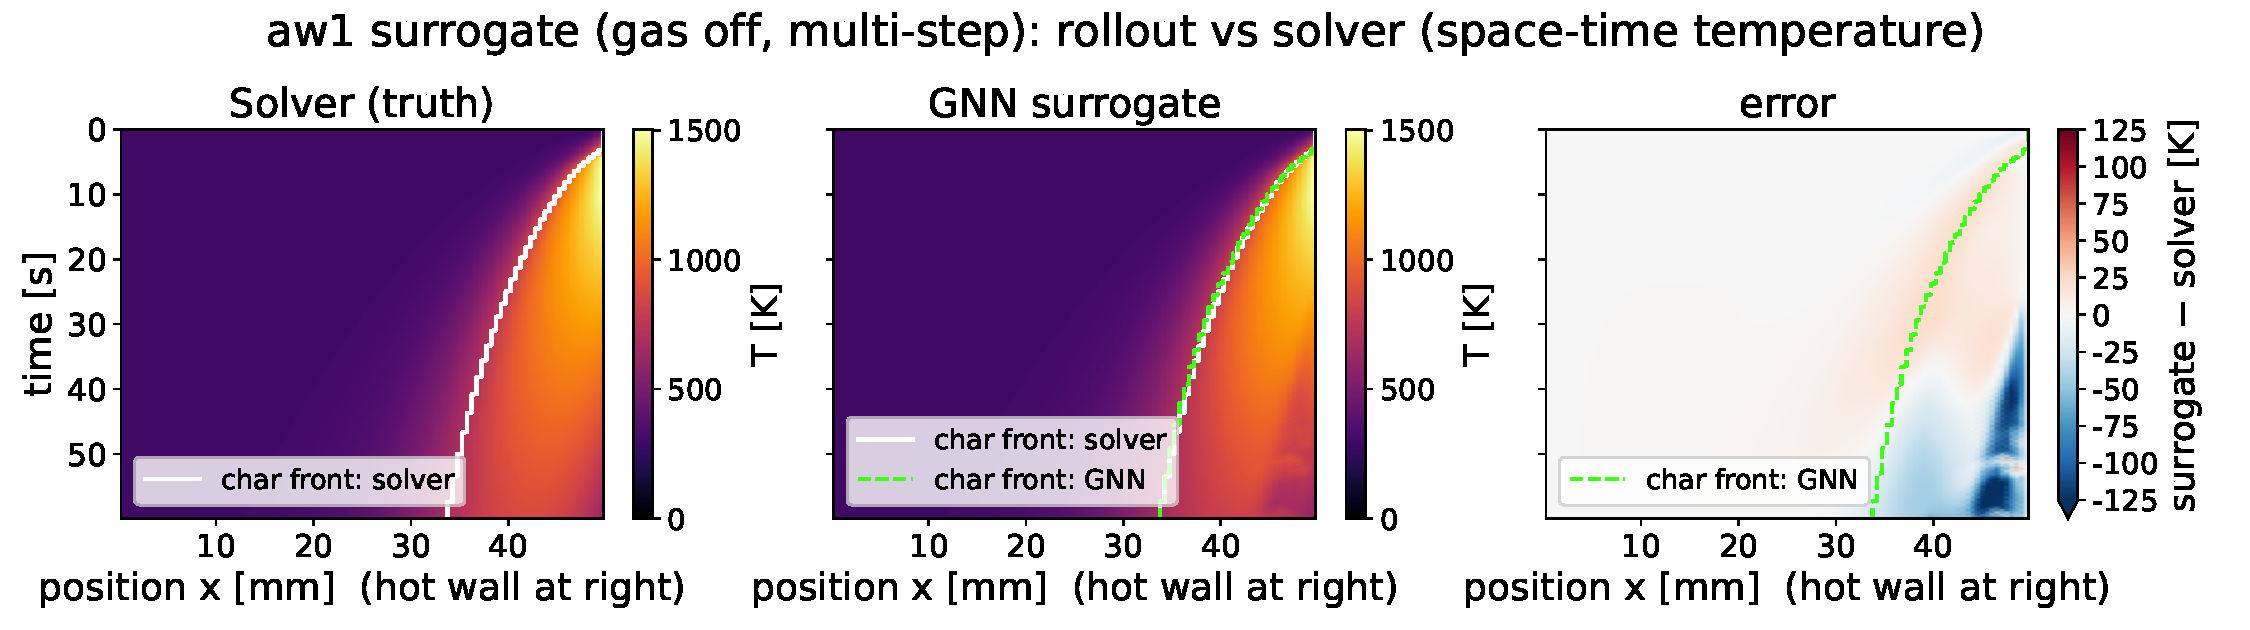
\includegraphics[width=\textwidth]{aw1/rllt_spt_signed.pdf}
  \caption{Gas-off (\texttt{aw1}) rollout: solver, surrogate, and error over 60~s.
  Mean error 7.6~K, char fronts (solver white, surrogate green) nearly coincident.}
  \label{fig:aw1}
\end{figure}

\subsection{The coupled case breaks it (aw2)}
The same approach fails on \texttt{aw2}, which adds the pyrolysis-gas transport and
the aerothermal surface. Trained the same way and rolled out on a held-out forcing,
the purely learned network diverges and reaches past a hundred thousand kelvin
(Fig.~\ref{fig:contrast}, right). The trouble is that \texttt{aw2} is much stiffer.
The aero flux switches on and off like a square pulse, so the surface temperature
jumps hundreds of kelvin in a single step, and the gas pressure and mass flux are
tightly coupled to the temperature. A network asked to learn all of that from
scratch has nothing to hold onto, and small per-step errors compound until the
rollout runs away.

\begin{figure}[t]
  \centering
  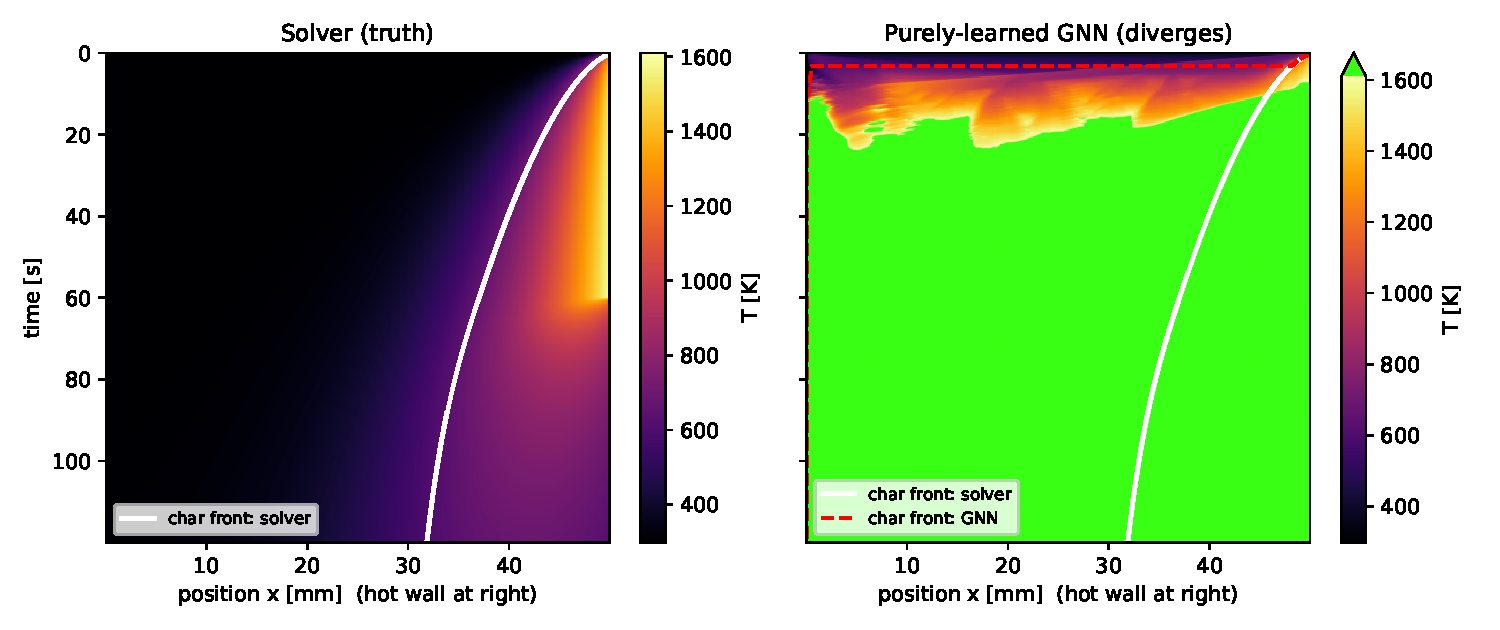
\includegraphics[width=0.667\textwidth]{aw2/contrast_diverged.pdf}
  \caption{Held-out \texttt{aw2}, same forcing. Solver truth (left) and a purely
  learned network that diverges off scale (right, green).}
  \label{fig:contrast}
\end{figure}

\subsection{Building the physics in}
The fix is to stop asking the network to learn what is already known
(Fig.~\ref{fig:arch}). Three pieces of
physics are built into the update instead of learned. First, the pyrolysis uses the
solver's own per-species Arrhenius kinetics, unchanged. Second, the conduction rate
$D$ is anchored to its physical value. Third, each conduction update is written as a
bounded average of a cell and its neighbors, a conservative flux exchange across the
faces. The conduction update for a field value $u$ is
\begin{equation}
  u_i \;\leftarrow\; u_i + \sum_{j} c_{ij}\,(u_j - u_i),
  \qquad c_{ij} \ge 0, \quad \textstyle\sum_j c_{ij} \le 1,
\end{equation}
where $u_i$ is the value at cell $i$, each $u_j$ is a neighbor, and the non-negative
weights $c_{ij}$ sum to at most one and are set by $D$. The update is a weighted
average of the cell and its neighbors. The new value stays within the range of its
neighbors, the discrete maximum principle, so the field can never grow beyond its
surroundings and cannot blow up. With these in place the network only has to learn
the small remaining piece, the coupling from the gas state to the decomposition
rate, a handful of parameters. This structured surrogate is stable, and it
reproduces the held-out gas case to about 25~K. Structuring the physics in is what
makes the gas case work at all.

\begin{figure}[H]
  \centering
  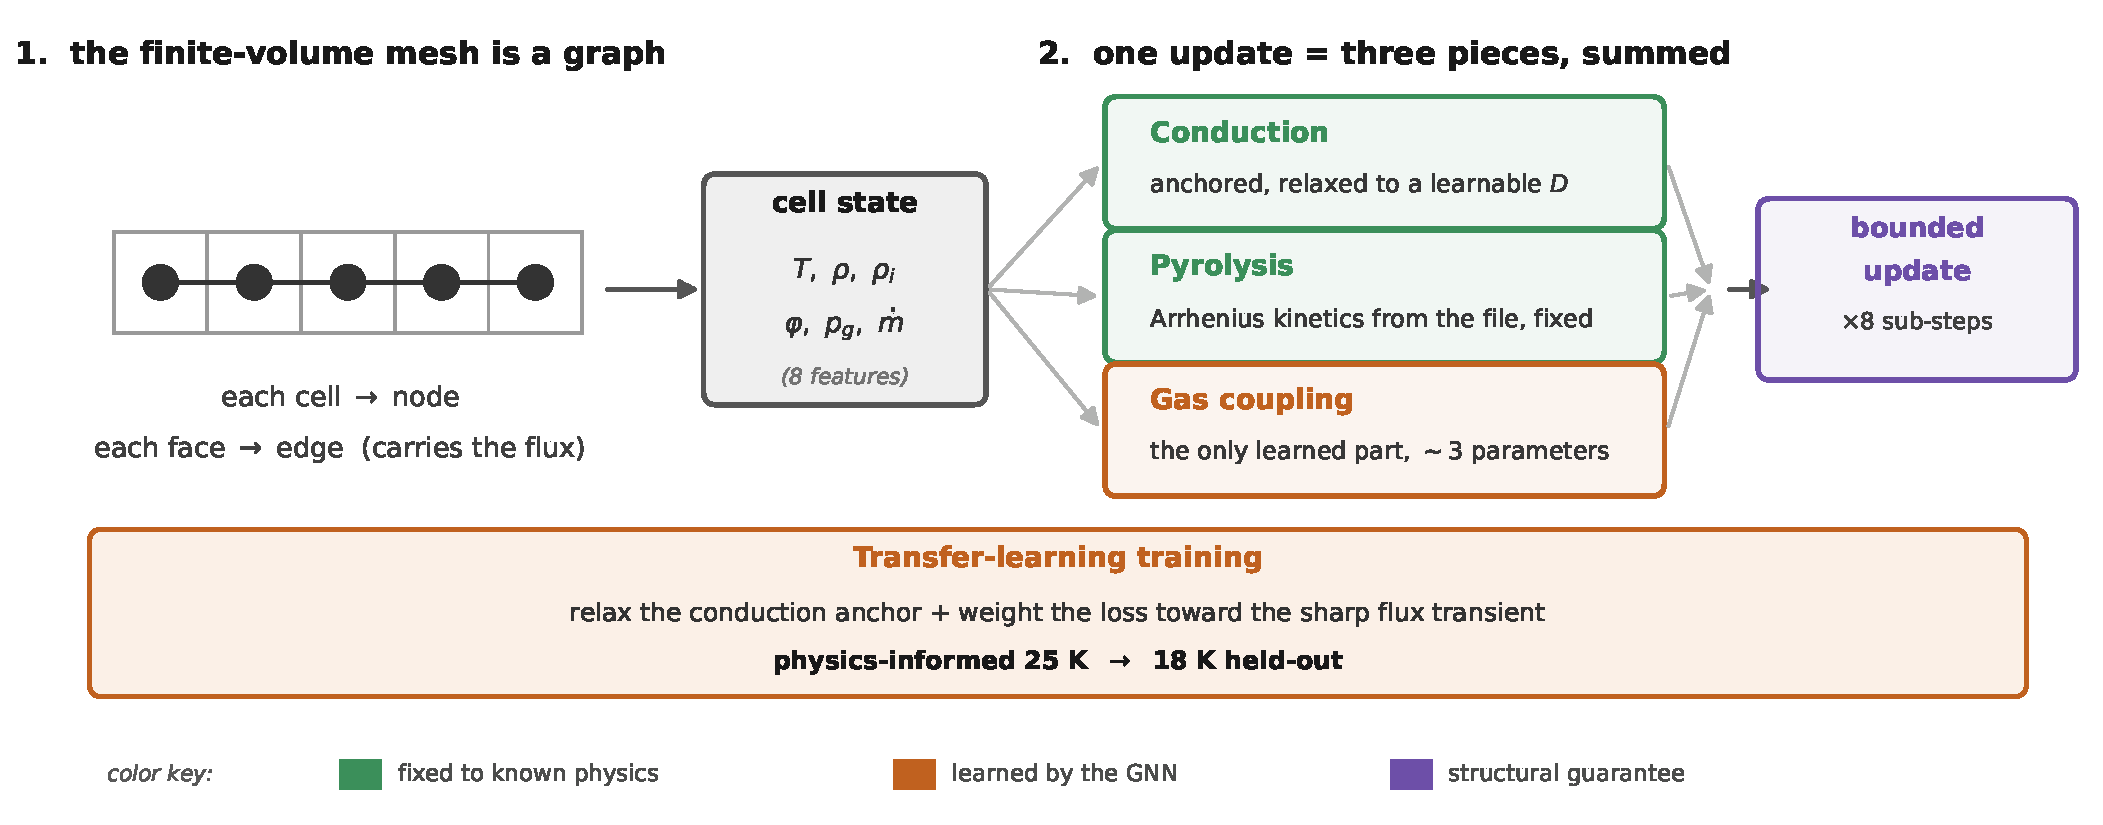
\includegraphics[width=\textwidth]{gnn_arch.pdf}
  \caption{The physics-informed surrogate: known physics is built into the update and
  only the small gas coupling is learned, inside a bounded exchange that cannot blow
  up.}
  \label{fig:arch}
\end{figure}

\subsection{Borrowing a transfer-learning trick}
The last gain comes from a transfer-learning idea used in a recent physics-informed
neural network study~\cite{cao2026}. The error in the structured model sits mostly at the sharp
flux transient, so two changes concentrate the model's effort there. First, the
conduction anchor is relaxed. Instead of holding the conduction rate fixed, the model
is allowed to adjust it during training, starting from the physical value. Second,
the training loss is weighted toward the cells that change the most from one step to
the next, which are exactly the ones near the flux switching on and off. On their
own, neither change helps much. The weighting has nothing to adjust while the
conduction is frozen. Once the conduction is free to move, the transient-focused
training has room to work, and the two together bring the held-out error down to
about 18~K. The error falls to about 8~K by the end of the rollout, the surrogate
stays bounded to the solver's own temperature range throughout, and it tracks the
char front to about one millimeter. The learned conduction settles at 0.336 against
the physical anchor of 0.375, close to the physics but fine-tuned to the data. This
is the final model (Fig.~\ref{fig:aw2}).

\begin{figure}[t]
  \centering
  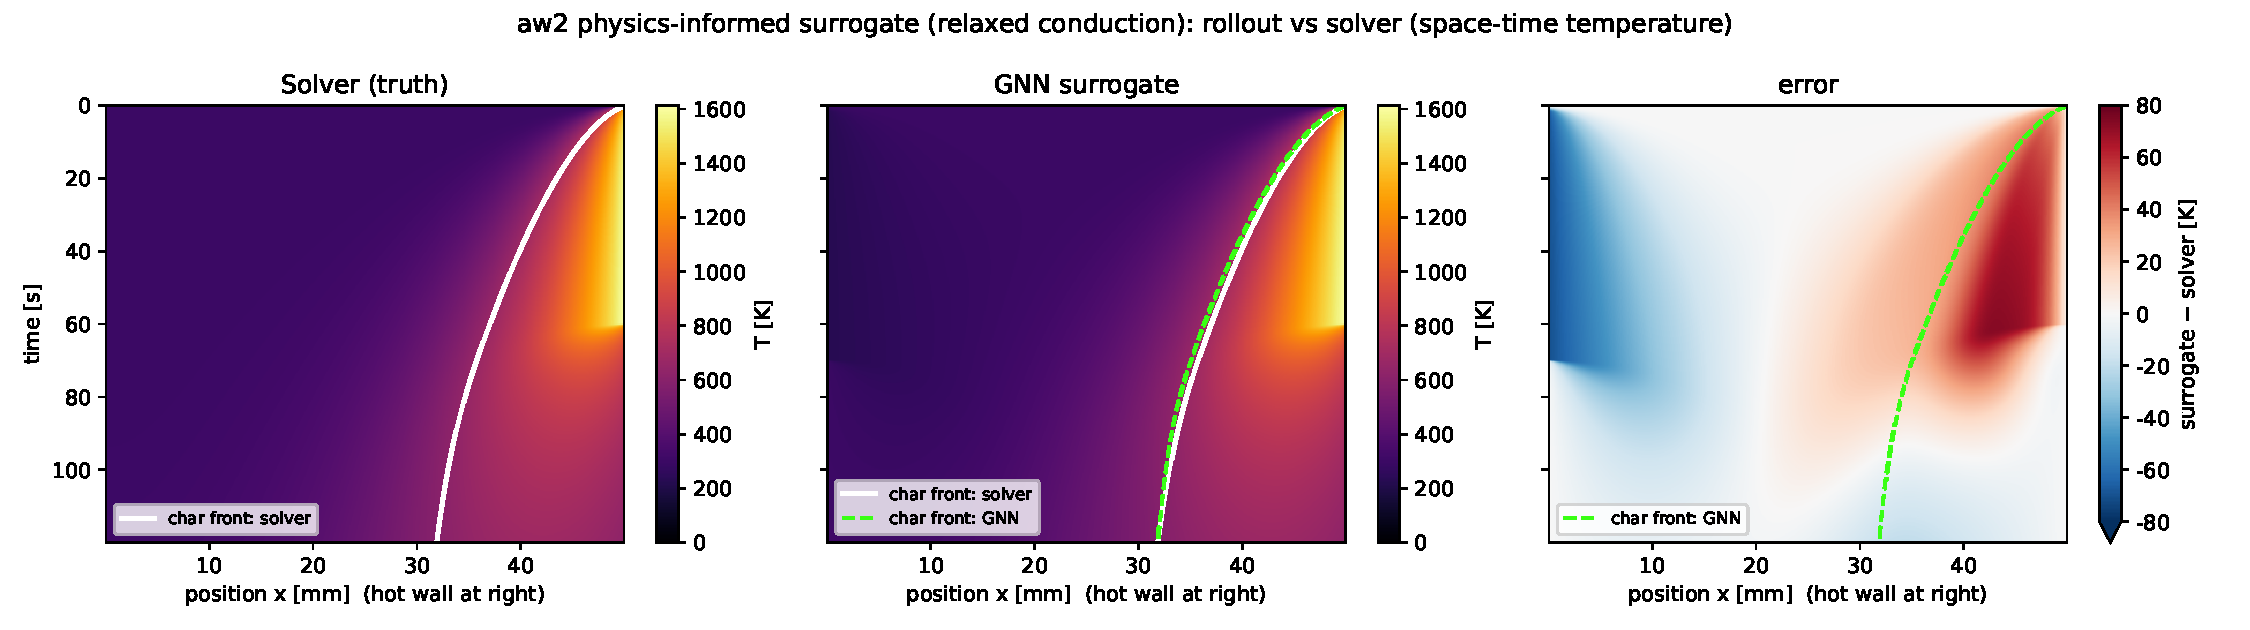
\includegraphics[width=\textwidth]{aw2/rllt_spt_signed.pdf}
  \caption{Gas (\texttt{aw2}) physics-informed rollout: solver, surrogate, and error
  over 120~s. Mean error 18~K, char fronts nearly coincident.}
  \label{fig:aw2}
\end{figure}

\subsection{Speed}
On the held-out 120~s gas case the surrogate
completes its rollout in about 92~seconds on a single GPU and about 100~seconds on
a CPU. The Python solver takes about 925~seconds on the same case, and the compiled
Fortran takes about 180~seconds. So the surrogate is roughly ten times faster than
the Python solver and almost twice as fast as the compiled Fortran, on either a CPU
or a single GPU. The advantage is modest at this 1D scale, where the mesh is small
and the per-call cost of the network is not amortized. The larger gains this
approach targets come from running many design cases together and from the steeper
per-step cost of higher-dimensional solvers.

\section{Training Data and Port Validation}
\subsection{Choosing the training data}
A surrogate is only as good as the states it has seen. A graph neural network learns
a local update, how a cell changes given itself and its neighbors, so it needs
training data that covers the range of conditions it will face and that stays
physically consistent.

I generate the data by running the validated Python solver across a sweep of aerothermal
forcings, each a different flux history, and recording the full field over time as a
trajectory. For \texttt{aw2} the sweep is twenty-four forcings, and a separate unseen
forcing is held out to test generalization. The recording is at a fine cadence, so
the sharp flux transient is captured rather than averaged over.

Two choices matter. First, the data comes from real solver trajectories rather than
randomly sampled states. Temperature and char state are tightly coupled in a
pyrolyzing material, and a real trajectory keeps them on that physical manifold.
Sampling the two independently would produce impossible states, such as a hot but
still-virgin cell, and training on those destabilizes the rollout. Second, the sweep
spans a range of forcings rather than a single case, so the surrogate learns the
response across conditions instead of memorizing one history.

\subsection{Validation of the Python port}
The data is only useful if the port that generates it is faithful, so the port is
validated column by column against the Fortran output from a run with the same
configuration. On \texttt{aw1} every output column matches to about $10^{-8}$,
machine precision. On \texttt{aw2\_tc21}, with the gas physics on, the temperatures
match to a maximum of 0.064~K and the hot aerothermal surface to 0.06~K
(Table~\ref{tab:val}). That agreement is why the data can be trusted to train the
surrogate.

\begin{table}[H]
\caption{Port validation against the Fortran reference (\texttt{aw2\_tc21}).}
\label{tab:val}
\centering
\begin{tabular}{ll}
\toprule
Quantity & Agreement \\
\midrule
All temperature columns & max 0.064~K, mean $\sim$$4\times10^{-4}$~K \\
Hot aerothermal surface & 0.06~K \\
Densities & $\sim$$10^{-3}$ to $10^{-9}$ \\
Time, cold back face & bit-exact \\
\bottomrule
\end{tabular}
\end{table}

\section{Discussion and Open Questions}
Two points are worth drawing out. First, the coupled gas case needs its known
physics built into the surrogate. A purely learned network diverges there, and
anchoring the conduction and the Arrhenius kinetics to the reference solver is what
makes it work. Second, a domain-averaged error can look small while hiding an
unphysical field, so I track the char-front depth rather than the mean when judging
whether a surrogate rollout is faithful. I define the char front as the deepest point at which the reactive
density has fallen below 98\% of its virgin value, a chosen reference threshold
marking the onset of decomposition. The same threshold is read from the solver and
the surrogate, so the comparison is on one yardstick, and the agreement between the
two fronts does not depend on the exact cutoff.

One question about the shipped cases. As it ships, \texttt{aw2\_tc22} is
byte-for-byte identical to \texttt{aw2\_tc21}. It has the same \texttt{heat.case},
the same \texttt{tc\_locations.dat}, and the same flux file, and its
\texttt{CASE\_NAME} field still reads \texttt{'aw2\_tc21'}. So it does not add an
independent validation condition. Was \texttt{tc22} meant to carry a different
configuration, for example a different flux history or different thermocouple
depths? Knowing that would let me treat 2.1 and 2.2 as two cases rather than one.

\section{Conclusion}
The 1D heat-shield solver can be reproduced faithfully in Python, to machine
precision on the conduction-pyrolysis case and to 0.064~K on the full gas case, and
a graph neural network trained on that data is a fast and faithful surrogate. On
the coupled gas case it reproduces a held-out history to about 18~K, tracks the
char front to about a millimeter, and runs almost twice as fast as the compiled
Fortran solver. The next steps are to generalize across mesh resolutions, to measure the
speedup across a full design-relevant batch of runs, and to extend the physics with
radiation and surface recession.

\bibliographystyle{unsrt}
\bibliography{heat_gnn_refs}

\end{document}
